%% LyX 2.1.0dev created this file.  For more info, see http://www.lyx.org/.
%% Do not edit unless you really know what you are doing.
\documentclass[english,conference]{IEEEtran}
\usepackage[T1]{fontenc}
\usepackage[latin9]{inputenc}
\usepackage{amsmath}
\usepackage{amssymb}
\usepackage{stmaryrd}
\usepackage{graphicx}

\makeatletter

%%%%%%%%%%%%%%%%%%%%%%%%%%%%%% LyX specific LaTeX commands.
%% Because html converters don't know tabularnewline
\providecommand{\tabularnewline}{\\}

%%%%%%%%%%%%%%%%%%%%%%%%%%%%%% User specified LaTeX commands.


% manually specify the path to it: e.g.,
% \documentclass[conference]{../sty/IEEEtran}

\usepackage{times}\usepackage{psfig}% Add all your packages here

% correct bad hyphenation here
\hyphenation{op-tical net-works semi-conduc-tor IEEEtran}

\IEEEoverridecommandlockouts    % to create the author's affliation portion
                % using \thanks

\textwidth 178mm    % <------ These are the adjustments we made 10/18/2005
\textheight 239mm   % You may or may not need to adjust these numbers again
\oddsidemargin -7mm
\evensidemargin -7mm
\topmargin -6mm
\columnsep 5mm

\makeatother

\usepackage{babel}
\begin{document}
% paper title: Must keep \ \\ \LARGE\bf in it to leave enough margin.



\title{\ \\
 \textbf{A Fuzzy/Probabilistic Approach to Uncertain Interval Algebra}}


\author{Keyvan Mir Mohammad Sadeghi and Ben Goertzel}

\maketitle
% make the title area

\begin{abstract}
A novel approach to uncertain temporal inference is presented. Allen's
Interval Algebra is extended to fuzzy time-intervals via representing
the latter as trapeziums with distinct beginning, middle and end.
An uncertain version of the Interval Algebra composition table is
developed via running a computer simulation in which a large number
of fuzzy time-intervals are drawn from an assumed probability distribution,
and using machine learning to induce uncertain compositional rules
that hold approximately across the corpus of simulated intervals. 
\end{abstract}
% no key words



\section{Introduction}

\PARstart{B}{en} can write a couple intro paragraphs \cite{PLN}


\subsection{Allen Interval Algebra}

One way to approach temporal reasoning is to represent the events
as \emph{intervals}. An interval captures some portion of time within
which some qualities hold. Any temporal event could be represented
as \textbf{{[}a, b{]}} where \emph{a} is the beginning of the event
and \emph{b} is the ending. There has been many works focused on addressing
interval handling in temporal inference, most notable of these are
Allen's Interval Algebra (IA) \cite{Allen} and Interval Temporal
Logic (ITL) \cite{Moszkowski-Thesis,Moszkowski-Paper}. 

tfyrtfyrty

\begin{tabular}{|c|c|c|}
\hline 
Precedes (p) & Meets (m) & Overlaps (o)\tabularnewline
\hline 
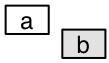
\includegraphics[scale=0.4]{p} & 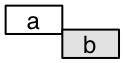
\includegraphics[scale=0.4]{m} & 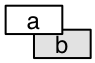
\includegraphics[scale=0.4]{o}\tabularnewline
\hline 
Preceded By (P) & Met by (M) & Overlapped By (O)\tabularnewline
\hline 
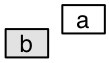
\includegraphics[scale=0.4]{pi} & 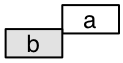
\includegraphics[scale=0.4]{mi} & 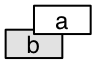
\includegraphics[scale=0.4]{oi}\tabularnewline
\hline 
Finished By (F) & Contains (D) & Starts (s)\tabularnewline
\hline 
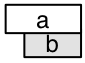
\includegraphics[scale=0.4]{fi} & 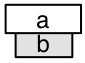
\includegraphics[scale=0.4]{di} & 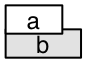
\includegraphics[scale=0.4]{s}\tabularnewline
\hline 
Finishes (f) & During (d) & Started By (S)\tabularnewline
\hline 
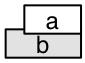
\includegraphics[scale=0.4]{f} & 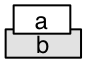
\includegraphics[scale=0.4]{d} & 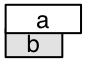
\includegraphics[scale=0.4]{si}\tabularnewline
\hline 
\multicolumn{1}{c|}{} & Equals (e) & \multicolumn{1}{c}{}\tabularnewline
\cline{2-2} 
\multicolumn{1}{c|}{} & 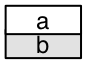
\includegraphics[scale=0.4]{e} & \multicolumn{1}{c}{}\tabularnewline
\cline{2-2} 
\end{tabular}


\subsection{Fuzzy Interval Algebra}

Keyvan should summarize prior papers on Allen Interval Algebra, with
references

Keyvan should briefly explain why we didn't just use their work


\section{A Trapezium Model of Fuzzy Intervals}

Keyvan will explain the modeling of events as trapeziums with beginning,
middle and end, including a pretty diagram of a trapezium


\section{Defining Fuzzy Interval Relations via Convolution}

Keyvan will describe the convolution approach to fuzzy interval relations,
preferably using a diagram illustrating one example (could be transitivity
of \textquotedbl{}precedes\textquotedbl{})


\section{Probabilistic Estimation of a Fuzzy Interval Relation Composition
Table}

Keyvan will explain the approach to generating a composition table
probabilistically

A graph illustrating the transitivity of precedence rule should be
presented, because 3D graphs are pretty and shiny

We can give example results on the precedence rule, and leave full
discussion of the composition table till later..

\bibliography{allen}
 \bibliographystyle{plain}

% that's all folks

\end{document}
